\chapter{Developer's Documentation}

In this chapter, we will examine the structure of our game and the implementation of its
various modules. The source code of the game is a part of Attachment A and can be compiled using Visual Studio 2015 Community.
In Figure~\ref{engine-layout}, we can see the main modules of the engine of our game and their relationships.

\begin{figure}[H]
    \centering
    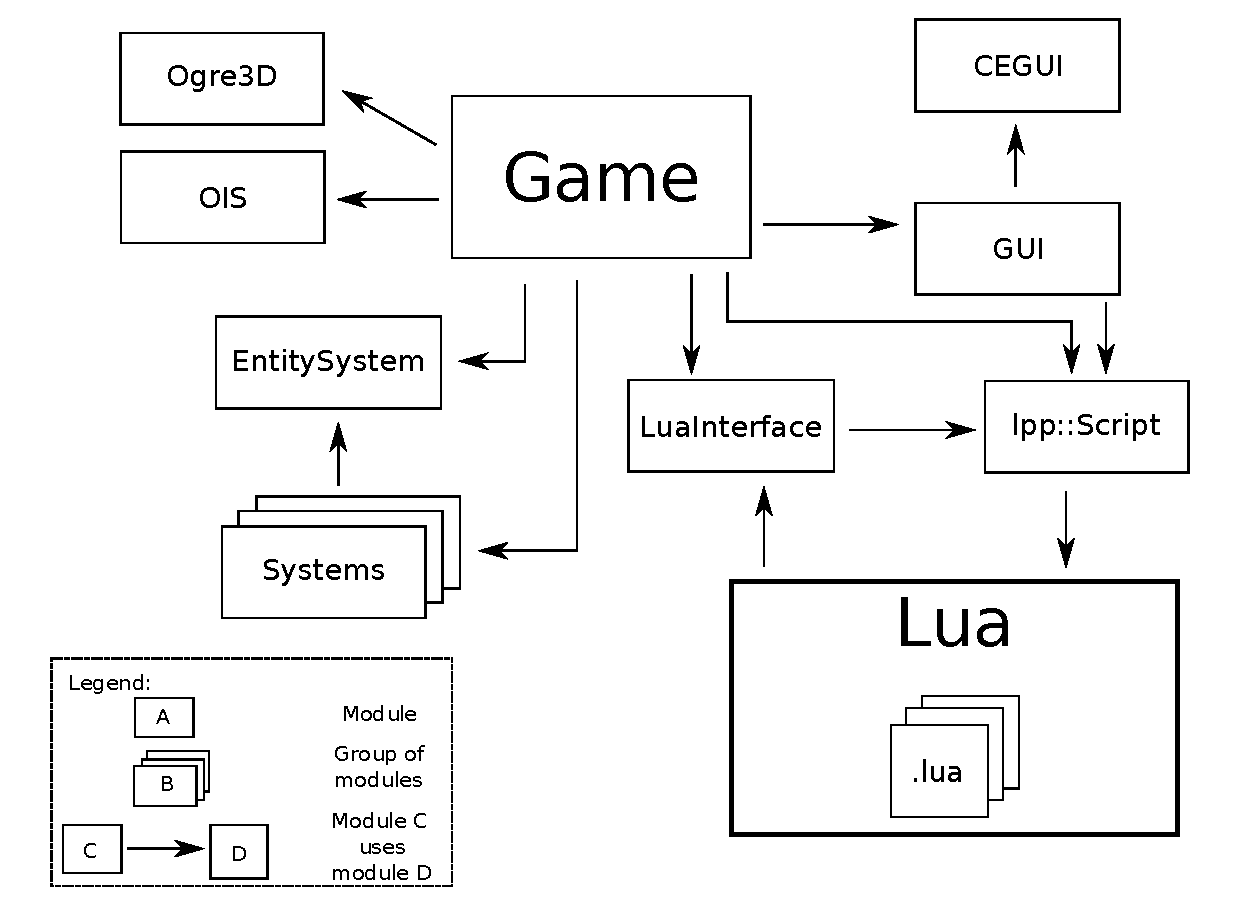
\includegraphics[width=\columnwidth]{../img/engine.pdf}
    \caption{Core of the game's engine.}
    \label{engine-layout}
\end{figure}

The central part of our engine is the \texttt{Game} class, which performs initialization of all modules, game updates and handles events
passed to it by two of our libraries -- Ogre3D, which is used for graphics, and OIS\footnote{Bundled with Ogre3D.}, which is used for
text input. These two libraries are directly used by the engine, but the remaining two -- CEGUI and Lua -- use special interface modules
that wrap and use their API.

The GUI module, which acts as an interface for CEGUI, comprises the \texttt{GUI} class and various different classes that represent
different windows that are part of our user interface.

Lua uses different classes for the different directions of communication. When the engine accesses Lua, it uses
the \texttt{lpp::Script} class, which acts as a wrapper facade over the Lua~C~API. When, on the other hand, Lua accesses parts of the
engine it uses the \texttt{LuaInterface} class, which binds functions of the engine that are written in \cpp to Lua, creating our
modding API.

The update logic of the game is performed by systems which, with the exception of \texttt{EntitySystem}, are equal in functionality.
\texttt{EntitySystem} stands out because it, besides updating the game, aslo acts as a component manager and provides components
to the rest of the systems.

In the following sections we will examine these main modules of the engine as well as various other modules, which mostly serve as tools
to the main modules.

\section{Game}

The \texttt{Game} class is the central part of our engine. In its constructor, every module of the engine -- that needs initialization --
is initialized. This class also serves as the main connection between the Ogre3D and OIS libraries and our engine.It does so by inheriting
four listener classes from these libraries -- \texttt{Ogre::FrameListener}, \texttt{Ogre::WindowEventListener}, \texttt{OIS::KeyListener}
and \texttt{OIS::MouseListener}.

Communication between the game and these two libraries is done, besides using their API, by overriding virtual functions of these classes
which act as event handlers. We can see these functions in Listing~\ref{ois-ogre-callbacks}. While names of most of these functions are
self-explanatory -- and their documentation can be found in the Ogre3D and OIS documentations -- we will examine the functionality of
\texttt{frameRenderingQueued} in a bit more depth.

\begin{listing}[H]
    \centering
    \begin{lstlisting}[language=C++]
// Ogre3D
bool frameRenderingQueued(const Ogre::FrameEvent&);
void windowResized(Ogre::RenderWindow*);
void windowClosed(Ogre::RenderWindow*)

// OIS
bool keyPressed(const OIS::KeyEvent&);
bool keyReleased(const OIS::KeyEvent&);
bool mouseMoved(const OIS::MouseEvent&);
bool mousePressed(const OIS::MouseEvent&,
                  OIS::MouseButtonID);
bool mouseReleased(const OIS::MouseEvent&,
                   OIS::MouseButtonID);
    \end{lstlisting}
    \caption{Virtual functions overriden in the \texttt{Game} class.}
    \label{ois-ogre-callbacks}
\end{listing}

\texttt{Ogre::FrameListener} provides three virtual functions -- \texttt{frameStarted}, which is called when a frame
is about to begin rendering, \texttt{frameEnded}, which is called when a frame has just been rendered, and \texttt{frameRenderingQueued},
which gets called when all rendering commands have been issued and are queued for the GPU to process. In our \texttt{Game} class, we override
only this last function -- although others can be overriden for different actions as well -- because while the GPU processes the current
frame, the CPU can be used for different tasks -- such as our update loop. This means that any changes that happen inside this function
will be rendered on the next frame, but in our game this delay is not noticeable as the player does not directly control any one entity.
We use this function to perform the main functionality of our game -- performing game update by calling the update functions of all
systems that are in the game.

Besides handling input and window events, this class contains several auxiliary functions related to initialization, level creation and
state changing. To see more information about these functions, refer to their documenting comments in the header file \texttt{Game.hpp} or
in the generated documentation.

\section{Components}

Component is a data aggregate that describes a specific characteristic of an entity that contains the component.
These components can describe various different characteristics. Components like \texttt{HealthComponent}, \texttt{ManaComponent}
or \texttt{GraphicsComponent} describe an attribute or a set of attributes of an entity. On the other hand, components like
\texttt{AIComponent} or \texttt{EventHandlerComponent} describe the behavior of an entity. Even the presence of a
component can express a characteristic -- e.g. \texttt{MineComponent} does not contain any data, but if an entity has this component, it
can be mined. In our engine, these
components are represented as simple structures with a name in the form of \texttt{<Characteristic>Component} and defined in the header file
\texttt{Components.hpp}. 

In Listing~\ref{component-ex}, we can see an example of a component -- the MovementComponent, which describes the speed of an entity.
Every component has a static integer field representing its type, which is used for communication between Lua and \cpp because Lua does not
understand the notion of templates, which we use for the different functions that manipulate with components, and as such it needs
to specify what kind of component should be used when it calls a \cpp function.

\begin{listing}[H]
    \centering
    \begin{lstlisting}[language=C++]
struct MovementComponent
{
    static constexpr int type = 4;

    MovementComponent(tdt::real speed = 0.f)
        : speed_modifier{speed}, original_speed{speed}
    { /* DUMMY BODY */ }

    tdt::real speed_modifier;
    tdt::real original_speed;
}
    \end{lstlisting}
    \caption{Simplified representation of the MovementComponent structure.}
    \label{component-ex}
\end{listing}

There is only one other requirement for components, which is that they always need to have a parameterless constructor
\footnote{A constructor that has default values for all its parameters will suffice.}. This is required because
we often create components by calling a \cpp function in Lua and then set its fields, which would be impossible without a constructor that
doesn't need any parameters. Also note that because of this approach, any strings passed to any parameterized constructor are considered
to be passed from Lua and as such are \textbf{moved} because the originals are supposed to be destroyed by Lua once the creation is complete.

Besides the two requirements, components can contain any data required by the entity characteristic they describe. In the examle, the
MovementComponent contains two fields of type \texttt{tdt::real}\footnote{One of two numeric types used in the engine that is defined
in the file \texttt{Typedefs.hpp}, the other being tdt::uint.}
-- speed\_modifier, which indicates the speed of an entity, and original\_speed, which is used
to restore the speed of an entity that has been affected by a slowing effect. Note that, to conform our
ECS representation, components should not contain functions and any logic should be done through systems.

\section{Systems}

A system is a class that performs a part of the games update. The game provides a common abstract parent class \texttt{System}, which is
used for easy iteration over all systems during the update of the game. In general, a system should operate over one or more types of
components, but the creation of systems that do not use components is also possible.

The update function of every system is called once per frame, but the individual systems often have inner time periods between updates.

\subsection{EntitySystem}

\texttt{EntitySystem} is the main system as, besides performing part of the game's update, it acts as a component database. This means that
it stores all component containers, which are represented as \texttt{std::map<entity\_id, component>}. Besides storing the components,
it also provides a set of function templates used for component manipulation.

Some of these function templates can be seen in Listing~\ref{es-comp-manip-ex}. They can be used to test if an entity has a component,
to retrieve a component
that belongs to an entity, add a new component -- using the parameterless constructor -- to an entity and remove a component from an entity,
respectively. In addition to these templates, each of them has a secondary non-templated version which takes an integer as a second parameter,
which corresponds to the type of the component -- these functions are then used from Lua.
To prevent code repetition, these functions use an array of pointers to the templated versions in which the pointer at any given index points
to the instances of these templated functions that have their type field equal to the index number.

\begin{listing}[h]
    \centering
    \begin{lstlisting}[language=C++]
template<typename COMP>
bool has_component(tdt::uint id);

template<typename COMP>
COMP* get_component(tdt::uint id);

template<typename COMP>
void add_component(tdt::uint id);

template<typename COMP>
void delete_component(tdt::uint id);
    \end{lstlisting}
    \caption{Examples of the templates using for component manipulation.}
    \label{es-comp-manip-ex}
\end{listing}

In addition to these public templates, one more important private template is defined in \texttt{EntitySystem} -- \texttt{load\_component}.
This function template accepts the identifier of an entity along with a name of a Lua table, which it will then use to load a component
with fields specified by the provided table.

Besides component storage and manipulation, this class also serves as a system. During its update, it deletes all components and entities
that were scheduled for deletion by the function \texttt{delete\_component}. The reason for this delayed delete is that if we deleted
components from their containers immediately in the delete call, we might invalidate iterators as the call may very well happen during
an iteration over a component container.

\subsection{CombatSystem}

The \texttt{CombatSystem} class performs the update of basic combat between entities -- that is, melee
\footnote{By melee we refer to close range combat as is common in many games.} and ranged combat excluding spells.
During its update, it checks the ability to attack of all entities that currently have an active combat target. This includes checking
if the target is in sight and in range. If an entity can attack, the system either performs applies its damage to its target if the
attack is of the melee type or creates a new projectile if the attack is of type ranged.
After updating the combat state of all entities that are currently fighting, the system updates the movement of all projectiles.

This system also performs a special kind of pathfinding which is used to find a path for an entity that is trying to escape from an attacker.
This pathfinding, unlike the general pathfinding that finds a path to the target, uses a queue and is performed once per frame. The reason for
this is that this pathfinding does not need to be performed immediately, while the general pathfinding is often used to check for the
existence of a path and as such needs to be finnished right after its start so that the return value can be used.

In addition to performing part of the game's update, \texttt{CombatSystem} provides two important types of functions -- querying for closest
entity that satisfies a condition, applying an effect to all entities in range that satisfy a condition.

\subsubsection{Conditions and entity querying}

Conditions are functors -- that is, structures that overload the function call operator -- which are used to test if an entity satisfies
a certain requirement. \texttt{CombatSystem} provides a function template that can be used to find the closest entity that satisfies
a condition.

\begin{listing}
    \centering
    \begin{lstlisting}[language=C++]
template<typename CONT, typename COND>
tdt::uint get_closest_entity(tdt::uint, COND&, bool);
    \end{lstlisting}
    \caption{Signature of the entity query function template.}
    \label{cond-ex}
\end{listing}

In Listing~\ref{cond-ex}, we can see the signature of this function template. Its template parameters are \texttt{CONT}, which specifies
the type of component container the function will be querying over, and \texttt{COND}, which specifies the condition functor. The function
takes the identifier of the entity that performs the query, instance of the condition functor and a boolean value determining if the
target has to be in sight and returns the identifier of the closest entity that satisfies the condition.

\subsubsection{Effects and their application}

In addition to entity querying, \texttt{CombatSystem} provides a function template that allows us to apply an effect to all entities
that satisfy a condition and are withing range. An effect, similarly to a condition, is a functor which is used to affect the entity
it is used on.

\begin{listing}
    \centering
    \begin{lstlisting}[language=C++]
template<typename CONT, typename COND, typename EFFECT>
void apply_effect_to_entities_in_range(tdt::uint, COND&,
                                            EFFECT&, tdt::real);
    \end{lstlisting}
    \caption{Signature of the effect applying function template.}
    \label{effect-ex}
\end{listing}

The signature of this function template can be seen in Listing~\ref{effect-ex}. Its template parameters are the same as the ones used
in entity querying with the addition of the parameter \texttt{EFFECT}, which specifies the effect functor. The function takes the
identifier of the entity that applies the effect, the condition the targets need to satisfy, the effect that will be applied to the
targets and the maximal range the targets can be from the applying entity.

\subsection{EventSystem}

\texttt{EventSystem} manages event handling as part of the game update. To do this, it uses two different components --
\texttt{EventComponent}, which represents an event, and \texttt{EventHandlerComponent}, which represents the ability of an entity
to handle events.

During its update, this system iterates over all events in the game and, if they are active -- finds a suitable entity that will
handle the event. Events can be of two types, either targeted or area events. An event is targeted if it has a valid entity
identifier in its \texttt{handler} field, otherwise it is an area event.

To request an entity to handle an event, the system checks if the entity can handle it by testing the event type in the entity's
\texttt{possible\_events} bitset field. Every \texttt{EventHandlerComponent} has a string field \texttt{handler}, which specifies
which Lua table contains the event handling function called \texttt{handle\_event}. The system then calls this event handling
function and passes the identifier of the handling entity and the identifier of the event to it, which causes the entity
to handle the event.

To handle a targeted event, the system simply finds the event's handler entity and requests event handling, but to handle an area event,
the system has to iterate over different event handlers that are within radius of the event, which is specified in the
\texttt{EventComponent}'s field \texttt{radius} and increases on every update call until the event is destroyed. The system requests
all of the suitable entities to handle the event until any one entity returns \texttt{true}, in which case it destroys the
\texttt{EventComponent} of the event. The reason for destroying the component and not the entity that represents the event is that
an entity that causes the event often gains the component so that the lifetime of the event is bound to the entity -- e.g. a falling
meteor can have an \texttt{EventComponent} of type \texttt{METEOR\_FALLING} and when the meteor hits the ground, both the meteor and
the event get destroyed since they are one entity.

\subsection{TaskSystem}

Similarly to how \texttt{EventSystem} manages event handling, \texttt{TaskSystem} manages task handling. It does so by iterating over
all entities that have \texttt{TaskHandlerComponent} and calling the \texttt{handle\_task} Lua function that is located in the Lua
table which is specified in the component's field \texttt{blueprint}. This Lua table also contains a function called \texttt{task\_complete},
which is used to check if the current task an entity that is iterated over has been completed, in which case the system requests
handling of the next task in the component's \texttt{task\_queue}.

Additionally, an entity that is handling a task can enter a busy state by returning \texttt{true} from its task handling function.
While an entity is marked as busy, no other task handling nor any AI updates will be performed until its current task is completed.

\subsection{GridSystem}

\texttt{GridSystem} manages nodes in the pathfinding graph and structures that are placed on them. During its update, it examines all
nodes that were either freed, which means that a structure on them has been destroyed, or unfreed, which means that a building was
placed on them. The system uses lists of freed and unfreed nodes to correct paths that were blocked by a strucute placed on a node
that was part of the path. Additionally, it manages all entities that have \texttt{AlignComponent}, which is used to change the models
of walls depending on their neighbours.

\subsubsection{Grid}

\texttt{Grid} is an auxiliary singleton class that provides an interface for grid node manipulation and monitoring, which acts as a
wrapper around a set of entity identifiers that belong to the different nodes in the pathfinding graph. Its main use are the lists
of freed and unfreed nodes that are used by \texttt{GridSystem}. In addition to these lists, \texttt{Grid} provides functions for graph
creation, placement of an entity on a random node and distribution of multiple entities on adjacent nodes -- which can be used to spawn
a group of entities next to each other.

\subsection{WaveSystem}

\texttt{WaveSystem} manages the progression of enemy waves that attack the player's dungeon. During its update, it tracks time passed
since the last enemy wave and starts the next wave if needed. The system can be in three different states:

\begin{itemize}
    \item \texttt{ACTIVE} state, during which  an enemy wave attacks the player's
        dungeon and the system spawns enemies on spawning nodes that were selected during level generation. After the player's minions destroy
        all enemies in the current wave, the system transitions into the \texttt{WAITING} state.
    \item \texttt{WAITING} state, during which the system simply tracks a timer until the next wave and changes back to the \texttt{ACTIVE}
        state once the timer runs out.
    \item \texttt{INACTIVE} state, during which the system is idle. This state is entered once the system depletes all waves or is paused.
\end{itemize}

To monitor the current state of the wave when the system is in the \texttt{ACTIVE} state, every spawned entity increments the entity
counter and the system adds \texttt{DestructorComponent} to it which specifies which function should be called when the entity dies.
This function then decrements the entity counter. When the counter reaches zero and all entities have been spawned, the wave ends and
the system transitions to either \texttt{WAITING} or \texttt{INACTIVE} state.

A specific sequence of waves is defined by a Lua table. The name of the current wave Lua table is stored in the variable private
\texttt{wave\_table\_}. This table contains functions that prepare the wave sequence and start and end the individual waves. This table,
along with a tutorial on how to create a new wave sequence can be found in Chapter~4.

\subsection{Miscellaneous Systems}

Now that we have examined the bigger systems that are included in the game, we will briefly explain the update logic of the remaining
systems, which generally perform simple tasks.

\begin{itemize}
    \item \texttt{AISystem} iterates over all entities that have a \texttt{AIComponent} and calls the Lua functions that update
        their behavior if they are not currently performing a task.
    \item \texttt{GraphicsSystem} was designed to manage all manual graphics. Explosions are the only manual graphics that are
        currently in the game so the system updates the dimensions of all entities that have a \texttt{ExplosionComponent} and destroys
        them once they reach their limits.
    \item \texttt{HealthSystem} removes all entities that are marked as not alive and periodically regenerates their health.
    \item \texttt{InputSystem} handles the input from the player and uses it to control all entities that have a \texttt{InputComponent}.
    \item \texttt{ManaSpellSystem} regenerates mana of entities that have a \texttt{ManaComponent} and manages the spell casting of
        all entities that have a \texttt{SpellComponent}.
    \item \texttt{MovementSystem} manages the movement of all entities that have \\ a \texttt{MovementComponent} and are currently on a path.
        Note that this excludes homing projectiles, which are updated by the \texttt{CombatSystem}.
    \item \texttt{ProductionSystem} manages the production of entities by buildings. It tracks time periods between spawns and the spawn
        limit of a building and when the time comes and the spawn limit is not depleted, the system spawns a new entity
        either on the building if its just a tile on the ground or around the building if its solid and cannot be stood on.
    \item \texttt{TimeSystem} manages the different timers in the game, including, but not limited to the timers of \texttt{OnHitComponent},
        \texttt{LimitedLifeSpanComponent} and \texttt{TriggerComponent}. Additionally, it manages a special kind of events that are
        represented by a \texttt{TimeComponent}. These components can start or end events represented by a \texttt{EventComponent} or
        call Lua functions.
    \item \texttt{TriggerSystem} manages entities that have a \texttt{TriggerComponent} such as traps or portals. It checks all entities in
        range to see if they can trigger the entity with the \texttt{TriggerComponent} and if they can, calls the trigger function.
\end{itemize}

\section{lpp::Script}

The \texttt{Script} singleton class in the namespace \texttt{lpp} is a wrapper facade around the Lua C API which provides an easy to use
interface for communication between \cpp and Lua. It provides functions that allow us, for example, to execute Lua code passed as a string,
register \cpp functions to Lua, retrieve values from Lua and call Lua functions from \cpp. In addition to this wrapper, the \texttt{lpp}
namespace contains the \texttt{Exception} class. Besides the conventional \texttt{what} function, which returns a string describing the
nature of the exception, this class also has the \texttt{lua\_what} function, which returns the text of the Lua error that occured.

\section{LuaInterface}

\texttt{LuaInterface} is a static class that contains functions that are part of our modding API and is used for simple initialization
of the API. The reason for it being static is that Lua does not understand the notion of a function bound to an instance of a class
and as such can bind only static functions.

During the initialization of our API, arrays of pairs of function names and function pointers are registered in Lua. Each of
these arrays is then represented as a Lua table which contains the registered functions.
To register a function pointer, it is required by Lua to have the signature of \texttt{int (*name)(lua\_State*)}. Because of this,
\texttt{LuaInterface} contains static functions with this signature that act as wrappers around the actually called functions.

Listing~\ref{lua-api-ex} contains an example of such wrapper. In this wrapper, we first need to retrieve the actual parameters for our
functions. These parameters are located on the Lua stack -- i.e. in reversed order -- and we can use one our five macros for easy
parameter retrieval defined in the \texttt{LuaInterface} source file. In this example, we use \texttt{GET\_UINT} and \texttt{GET\_REAL},
each of which takes a pointer to the Lua state and an offset from the top of the stack. Once we retrieve these parameters, we can call the
wrapped function and push its result back onto the stack. Note that Lua supports multiple results from a function call and thus we can
push multiple values onto the stack. The amount of returned results is then returned from the wrapper.

\begin{listing}[H]
    \centering
    \begin{lstlisting}[language=C++]
int lua_wrapper_of_F(lua_State* L)
{
    tdt::uint param2 = GET_UINT(L, -1);
    tdt::real param1 = GET_REAL(L, -2);

    int result = F(param1, param2);
    lua_pushinteger(L, result);

    return 1;
}
    \end{lstlisting}
    \caption{An example of our modding API function implementation in \protect\cpp.}
    \label{lua-api-ex}
\end{listing}

\section{Helpers}

Helpers are auxiliary functions that are used for component manipulation that are placed within a namespace related to a specific component
-- e.g. the \texttt{HealthHelper} namespace contains functions that manipulate \texttt{HealthComponent}. These functions are mainly in the
form of a setter, which changes a field of the component after checking the validity of the new value, or getter, which returns the value
of a gield of the component or a default value if the component does not exist. But the body of these functions is not restricted and they
can perform any operation.

The main purpose of these functions is keep the \texttt{LuaInterface} class small, but can be used freely in \cpp as well if we need for
example parameter checking, default values or transaction logging. However, these functions generally retrieve the component from its
container and as such sequential calls to different helper functions of a single component will be slower than a direct manipulation
of the component.

\section{SpellCaster}

\texttt{SpellCaster} manages player spell casting. Player spells in our game can be of four different types -- \texttt{TARGETED}, which
affect a single selected target, \texttt{POSITIONAL}, which affect a specific area the player clicks at, \texttt{GLOBAL}, which have a
global effect on the game, and \texttt{PLACING}, which place a new entity into the game.

The spell casting process has two phases. Firstly, it selects the spell type and spell Lua table name and calls an initializating
function that is contained within the spell table. Secondly, it calls the casting function and passes parameters to it based on the spell
type when the player clicks on the screen to cast the spell.

This process is strongly connected to Lua, the \texttt{SpellCaster} class only manages spell changing and the two described phases, but
the effects of the spells are fully defined in Lua. In Section~4.5, we will examine the spell table and go over the spell creation process.

\section{Pathfinding}

In Section~2.6, we decided to use the A* algorithm for pathfinding in our game. While A* is the implemented algorithm, the game contains
a templated pathfinding system using functors for algorithms, heuristics and path types. This allows us to easily change the characteristics
of our pathfinding process. 

The \texttt{pathfind} function calls the algorithm functor, which has a static function \texttt{get\_path} that returns the found path.
After obtaining the path, \texttt{pathfind} resolves blocks that are placed on the path by requesting the entity that performs the
pathfinding to destroy them before continuing on its path. The algorithm functor is templated as well and its template parameter is
what we call a path type.

Path type is a functor that has a static function \texttt{return\_path}, which is called the first time a path is found and then whenever
an augmenting edge is found on the path. If the \texttt{return\_path} returns \texttt{true}, the path gets returned, and if it returns
\texttt{false}. Examples of such path types are the three path types that are implemented in the game -- \texttt{BEST\_PATH}, which forces
the algorithm to search the entire pathfinding graph, \texttt{FIRST\_PATH}, which terminates the algorithm the first time a path is found,
and \texttt{RANDOM\_PATH}, which acts as a compromise between the two aforementioned path types.

Lastly, both the \texttt{pathfind} function and the algorithm's \texttt{return\_path} function take a heuristic as a parameter. The heuristic,
unlike algorithm and path type, is not static as it in some cases requires to have a state -- for example, the heuristic used for running
away from an enemy needs to know the identifier of the enemy. The heuristic has a function \texttt{get\_cost}, which returns the
approximate cost of travel between two nodes in the pathfinding graph.

\section{Player}

\texttt{Player} is a singleton class primarily used for resource monitoring -- it stores information about the amount of all the player's
resources such as gold, mana, spawned entities and others. Additionally, it contains information about the starting state of the game,
such as initial spells and unlocked research. This is mainly used when we create a new game or when we load a previously saved game.

\section{Serialization}

The \texttt{GameSerializer} class is used to save the state of the game and to load previously saved states. It does so by creating Lua
scripts that use our API to change an empty level to the serialized one. For every entity, it iterates over all of its components and
outputs a sequence of API calls that add the component to the entity and restore the values of its fields. For this, the class has
an array of pointers to functions that serialize the different components indexed by the types of the components.

In addition to the component serialization, it also saves resources that are contained in the \texttt{Player} class, creates an empty
level, recreates the pathfinding graph, saves unlocked spells and buildings and the overall progress of the player's research.

To load a saved state of the game, it simply destroys all the entities in the game and resets the \texttt{Player} class to its initial state.
It then executes the serialized script to restore the state of the game.

\section{Tools}

In this section, we will examine some of the smaller tools that are used within the engine of our game.

\subsubsection{Camera}

The \texttt{Camera} class acts as a wrapper around the main \texttt{Ogre::Camera} instance. Its main purpose is to allow us control the
camera in multiple ways -- using both keyboard and mouse -- and it also allows us to change between the basic mode, in which the camera
has a fixed orientation, and the free mode, in which the player can move and rotate the camera freely in the game world.

\subsubsection{EntityPlacer}

\texttt{EntityPlacer} is used to place entities in the game world. To place an entity, we first need to call the function
\texttt{set\_current\_entity\_table}, which will change the entity that is currently being placed and show its model at the position
of the mouse cursor. While an entity is being placed, the game
will call the function \texttt{update\_position} which will move the temporary model to the specified position, which is used to make
the temporary model to follow the mouse cursor. Once the player clicks on a spot in the game world, the game calls the function
\texttt{place}, which will spawn a new instance of the entity that was placed at the current position of the placer.

\subsubsection{LevelGenerator}

Level generators, found in the namespace \texttt{level\_generators} are used to populate an empty game world with starting structures such
as buildings, walls and gold blocks. During the initialization of our game, the \texttt{Game} class creates an instance of the generator that
is defined -- using either \texttt{typedef} or \texttt{using} -- as \texttt{DEFAULT\_LEVEL\_GENERATOR} in this namespace.

This forces the constructor of any level generator to take a reference to the \texttt{EntitySystem} class and a \texttt{tdt::uint} because
the instantiation of the level generator is done generically with these two parameters. The reference to \texttt{EntitySystem} is used
for the creation of walls, blocks and others and the unsigned integer denotes the amount of iterations of the generation -- if the
level generator is iterative, otherwise this parameter may be ignored.

Any level generator has to also have a function with the signature \texttt{void generate(tdt::uint, tdt::uint, WaveSystem\&)}. This function
will then generate a level with dimensions equal to the passed integers and sets the spawn points for the passed wave system.

\subsubsection{RayCaster}

The Ogre3D library provides only a basic bounding box ray casting, but our walls do not have to fill their entire bounding box because of
alignment. For this, we used external code from the official Ogre3D website~\cite{Ogre3DRaycasting} in our \texttt{RayCaster} class
because of the author's limited knowledge of graphics programming. This class is used to check if two entities can see each other by creating
a ray between two points in the game world which, unlike standard Ogre3D ray casting, takes only actual models into account. The class
uses this ray to determine if there is a block between the two entities and if so, assumes they cannot seee each other because of this
block.

In Figure~\ref{los-problem}, we can see a situation where two ogres stand in front of each other and next to a diagonal wall. Because our
game world is made of tiles, the walls have the form of a cube and the diagonal wall is simulated using alignment, during which the wall
changes its model. However, even if the model is not a cube, the bounding box still is and because of this if we use Ogre3D ray casting
to determine if the two ogres can see each other, the result will be \texttt{false}. But since our \texttt{RayCaster} ray casts to
the polygon level, its use would yield \texttt{true} as the result.

\begin{figure}[h]
    \centering
    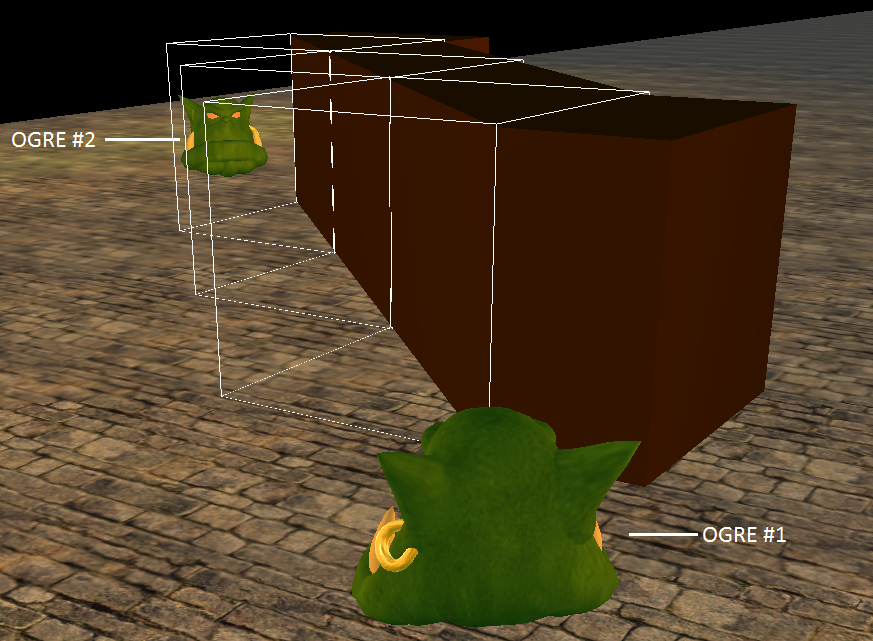
\includegraphics[width=\columnwidth]{../img/los-problem.png}
    \caption{An example situation where bounding box ray casting would not suffice.}
    \label{los-problem}
\end{figure}

\subsubsection{SelectionBox}

\texttt{SelectionBox} is a class used for entity selection using either the plane bounded volume query or ray casting provided by Ogre3D.
Whenever a player
clicks on anything in the game world -- besides parts of the GUI -- the \texttt{Game} class starts selection by setting the initial
point of the selecting square. Any mouse movement then sets the end point of the square so that the player has a visual feedback on his
selection. Once the player releases his mouse button, the query is executed on the created selection square to select all entities that
are located within it.

This class provides two modes of selection -- single selection and multi selection. The type used is determined by the size of the
selection square, so if the square is too small, a ray cast will be used instead of a volume query.

\section{GUI}

Our GUI module serves as a set of wrapper classes around CEGUI windows. The \texttt{GUI} singleton class is used for initialization and
shared control of all other windows -- e.g. to recursively toggle visibility of the windows. This class also contains instances of
most\footnote{It does not contain some testing windows, such as \texttt{EntityCreator}.}
of the other windows. Each of these windows inherits from \texttt{GUIWindow}, which provides common interface for visibility and
initializaion.

The game's GUI contains the following windows:

\begin{itemize}
    \item \texttt{Console} -- accepts Lua commands as its input and executes these commands in the Lua virtual machine.
    \item \texttt{EntityCreator} -- a window that allows the user to spawn entities by choosing them from the list of all
        available entities, mainly used for testing.
    \item \texttt{EntityTracker} -- display characteristics of the currently selected entity, e.g. its health or mana.
    \item \texttt{ResearchWindow} -- button based interface for research, the player can click on a research node if they have
        enough resources to unlock it.
    \item \texttt{BuilderWindow} -- provides the player with a selection of building they can build.
    \item \texttt{SpellCastingWindow} -- provides the player with a selection of spells they can cast.
    \item \texttt{GameLog} -- shows game messages, e.g. error messages when the player does not have enough resources
        to build a building.
    \item \texttt{MessageToPlayerWindow} -- a simple multi-purpose window with a message and buttons.
    \item \texttt{OptionsWindow} -- allows the player to change the game's resolution, toggle fullscreen mode and change key bindings.
    \item \texttt{TopBar} -- a small bar at the top of the screen that shows the player's current resources.
\end{itemize}
